\documentclass[40pt]{article}
\usepackage{multirow}
\usepackage{float}
\usepackage{graphicx}
\graphicspath{  }
\usepackage{wrapfig}
\usepackage{cite}
\usepackage{hyperref}

\begin{document}

\bigskip
\begin{center}
\Huge{\textbf{
PROJECT REPORT}}
\end{center}

\begin{center}
\huge{GROUP 19}
\end{center}

\begin{center}
\Large{\textbf{inficoders}}

 
 \end{center}
 \bigskip
 \vspace{1cm}
 \bigskip
 \begin{center}
 \Large{Rube Goldberg Machine}
 \\
 \Large{Simulation of 4 Stroke Combustion ~\cite{ref1} ~\cite{ref10} Engine With Gears}
 \\
 \large{by Naveen,Yathansh,Rajat}
 \end{center}
 \bigskip
 \begin{center}
 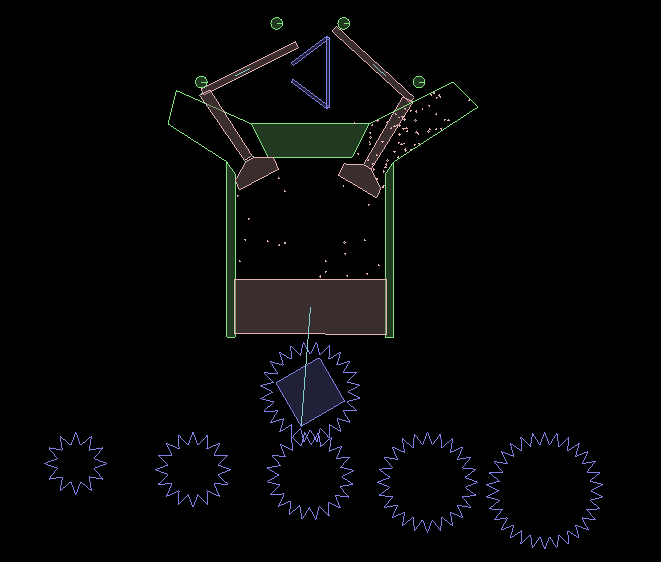
\includegraphics[scale=0.4]{pic1.png}\newline
 \newline
 \small{screenshot 4stroke combustion engine}
 \end{center}
 
 
 
 
\newpage




\begin{center}

\huge{
\textbf{Introduction\\}}
\end{center}
\Large
{
In this project, we have developed a simulation for the 4-stroke combustion engine. ~\cite{ref1} ~\cite{ref10} Along with the main engine, we have attached 5 speed gears to it, out
of which one can be attached to the engine at a time.
\\
}
\begin{center}
\huge
{
\textbf{Structure:\\}
}
\end{center}
\Large
{
The main body consists of the combustion engine. It has the following components:
\\
\begin{description}
  \item[$\bullet$ ]\textbf{ The Main Piston System\\}
  The main piston is the component which is used for the compression of the air in the compression chamber. This component is made up of a rectangular object, i.e., the piston, and the rotating square object which controls the motion of the piston. These two objects are attached with a distance joint.
This ensures that the up and down movement of the piston results in the rotation of the square object, and vice-versa. The piston is fixed horizontally inside the compression chamber by two stands on each side, and its vertical motion is fixed by the rotation of the square object. The square object has a main gear attached to it, which rotates with the same angular speed as the rotating square.
	\begin{center}
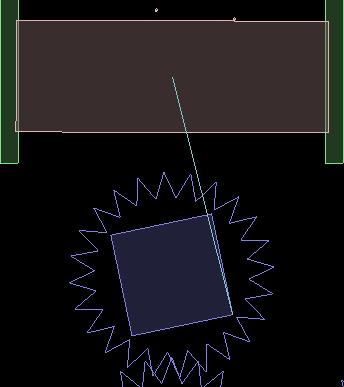
\includegraphics[scale=0.5]{mainPiston.png}\newline
\small{main piston}
\end{center}
    \item[$\bullet$ ] \textbf{The Left and Right valve System\\}
    The left and right valves are separate systems, and are dependent on gravity and a rotating triangle for their movement. the valves consist of three polygon-shaped objects attached with joints. The lowest part is a six-sided figure, and serves as the main part of the valve. The opening and closing of the valve depends upon the forward and backward motion of this object. The middle object is a rectangular stick attached singly to the lower object, and provides support for the motion of the lower object. Also, we have made use of the sensor data member, to make the middle object invisible to the air particles, and thus prevents any collisions there. The top object is another rectangular stick, which is attached doubly to the middle object. This double attachment makes the joint stiff and immovable and not rotatable. The density of this upper object is high, and it is pivoted at a point to the left of the centre of mass of this object. This fixed rotation at a point off-centre helps gravity determine the motion of the object, and hence the whole valve. There are two spherical fixed objects, which restrict the motion of the upper body.
The rotating triangle has an angular velocity with magnitude exactly half of that of the rotating square and direction opposite to it. The two upper parts of both the valves are predominantly forced by gravity to lean inside, keeping both the valves closed. Whenever the two vertices of the largest side of the triangle come in contact with these upper bodies, they force them to move in the opposite direction, forcing the valve to open for as long as the vertices and the sticks are in contact. This process is an important part of the 4-stroke cycle. The initial position of the rotating triangle is set up so that it is in sync with the motion of the piston, and hence is necessary for the completion of the 4-stroke cycle.\newline
\begin{center}
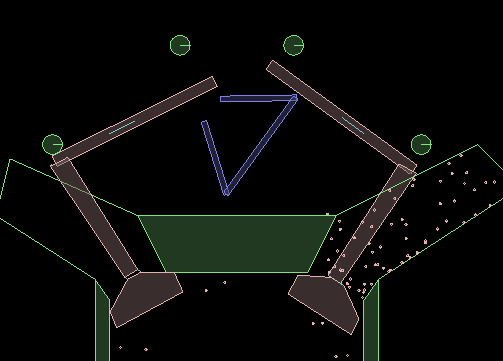
\includegraphics[scale=0.4]{valve.png}\newline
\small{valve system\\}
\end{center}
      \item[$\bullet$ ] \textbf{The Supporting Structures\\}
      The compression chamber is confined on both the sides by the left and the right stands, and from the top by a trapezoidal structure. These structures ensure that the compression chamber remains closed. Also the stands and the trapezoidal structure are placed such that they do fix the position of the
lower part of the valve in the closed-valve state.

        \item[$\bullet$ ] \textbf{The Inlet/Outlet Chambers and Air Particles}
        There are two chambers on the left and right of the compression chamber, which act as outlet and inlet respectively. The inlet chamber allows air particles to move to the compression chamber through the right valve. Similarly, the outlet chamber receives the compressed air from the compression chamber through the left valve. This completes the 4-stroke cycle. The air particles that are received in the outlet chamber are transported back to the inlet chamber. This ensures the continuation of the simulation. To accomplish this, we have implemented the contactListener class, and kept the last wall of the outlet as a contactListener object. Whenever an air particle comes into contact with this object, its coordinates are transformed, and it is transported back to the inlet chamber.
	\item[$\bullet$ ] \textbf{The Gears\\}
	There are 5 gears, and they are located below the combustion engine. At a particular time, exactly one of the gears is in contact with the main gear, that is attached to the rotating square object. All the gears have different sizes, but same size of spokes, thus resulting in different number of spokes on each gear. They are placed in increasing order of size and therefore number of spokes from left to right. This means that the rightmost gear is the first gear and the leftmost gear is the fifth gear. As it happens in real life, the first gear provides the least speed and maximum torque, whereas the fifth gear provides maximum speed and least amount of torque.
These gears are implemented by creating fixtures containing multiple lines, that are criss-crossed, thus giving the shape of the gears. We had to assign a fixed angle to each spoke in each gear, so that the size of the spoke remained same in all the gears. Correspondingly, the number of such spokes increased on increasing radius and angle for each spoke decreased.

\begin{center}
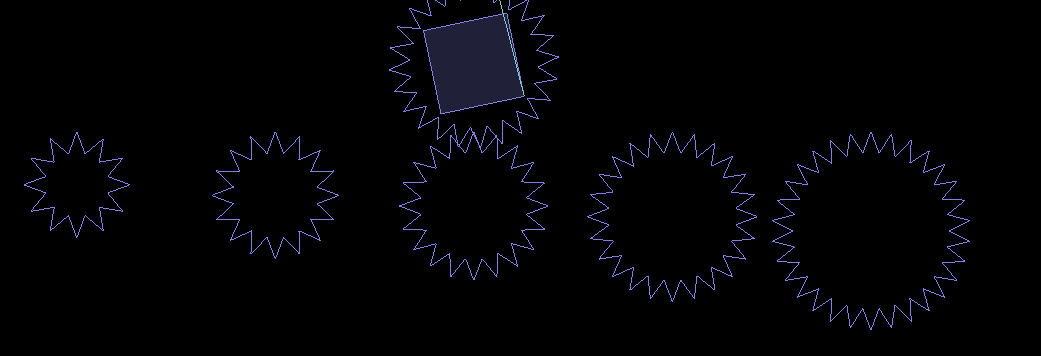
\includegraphics[scale=0.3]{gear.png}\newline
\small{gear}
\end{center}

\begin{center}
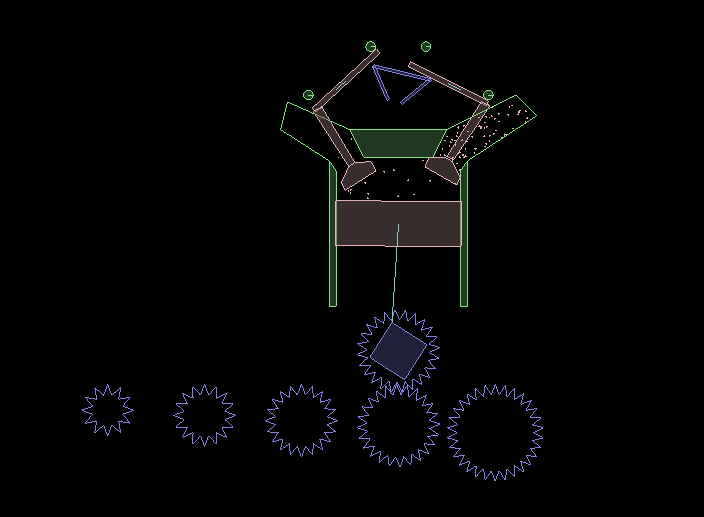
\includegraphics[scale=0.5]{pic2.png}\newline
\small{when air is compressed}
\end{center}
\end{description}


}


\begin{center}

\huge{
\textbf{Features\\}}
\end{center}
\Large
{
1) The speed of both the controlling gears can be increased or decreased by using the '+' and '-' keys on the keyboard. While high speed resembles an actual combustion engine, lower speed allows us to analyse and study the simulation carefully.\newline
\newline
2) Also, the gears can be shifted one at a time, by using the 'left' and the 'right' arrow keys. This is implemented by making the appropriate changes in the file 'callbacks.cpp'. We assigned functions to transform the co-ordinates of the gears based on the keyboard input.\newline
\newline
3) The process of reusing air molecules by their instantaneous transportation from outlet to inlet chamber is clever and remarkable.\newline
\newline
4) The creation of the gear-shaped object for gears, is a remarkable feat, since it was created by us.
\newline
}



\begin{center}

\huge{
\textbf{Limitations\\}}
\end{center}
\Large
{
1) At high speeds, the air molecules start "leaking" from the engine. This happens because (we found this as a plausible reason on the internet) Box2D has a certain interval after which it detects collisions. Then, if a collision occurs in between this interval, then Box2D is not able to detect it and it goes unnoticed. This results in the so-called "leaking" of air molecules. We could find no way of preventing this.\newline
\newline
2) The vertices of the rotating triangle should collide with exactly one of the two upper parts of the valves, and should remain invisible to other. We were not able to accomplish this, resulting in an extra opening and closing of the valves in one cycle. We tried to use the group index feature, to implement this, but met with some or the other error at all points.
\newline
\newline
3) The main rotating gear is a kinetic object. In its motion, it should collide with other gears, and cause them to move. But in our implementation, maybe because that shape was our own creation (again, this is only a plausible explanation we found on the internet), we could not make it interact with other objects, i.e., it became invisible to collisions. We could find no way to make it visible to collisions.
\newline
\newline
}




\begin{center}

\huge{
\textbf{Some Difficulties and How We Overcome Them\\}}
\end{center}
\Large
{
1) Any place where we required the use of concave/non-convex objects, we had to create smaller objects and join them. e.g. valves, rotating triangle.\newline
\newline
2) First we wanted to continuously create new air molecules and delete the molecules that reached the outlet. We tried many ways of doing this, but failed everytime. Then we found out about the contactListener class, and thus implemented a method to transport the air molecules from outlet back to the inlet.
\newline
\newline
3) We overcame the difficulty of the non-colliding nature of the main gear, by manually providing a function which kept the appropriate angular velocity of the gears, so that the rotation matched with that of the main gear.
\newline
\newline
}


\newpage

\begin{center}

\huge{
\textbf{Callgraph:Debug Mode\\}}
\end{center}
\begin{center}

\includegraphics[scale=0.04]{normalanalysis.png}\newline
\small{debug mode\\}
\end{center}

\begin{center}

\huge{
\textbf{Callgraph:Release Mode\\}}
\end{center}
\begin{center}

\includegraphics[scale=0.035]{releaseanalysis.png}\newline
\small{release mode\\}
\end{center}

\begin{center}
\Large{zoomed callgraph of release mode are as follows:\newline}
\end{center}


\begin{center}
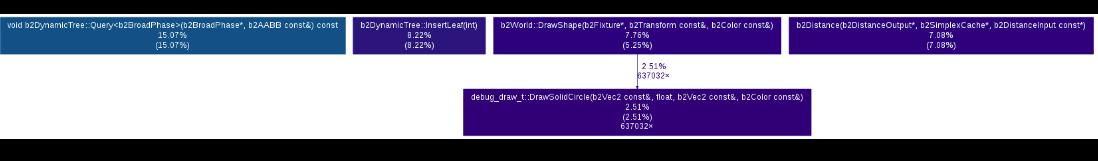
\includegraphics[scale=0.4]{release1.png}\newline
\small{release mode\\}
\end{center}


\begin{center}
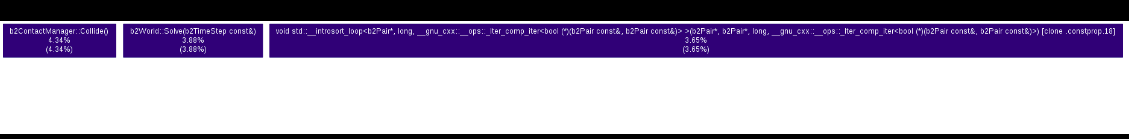
\includegraphics[scale=0.4]{release2.png}\newline
\small{release mode\\}
\end{center}


\begin{center}
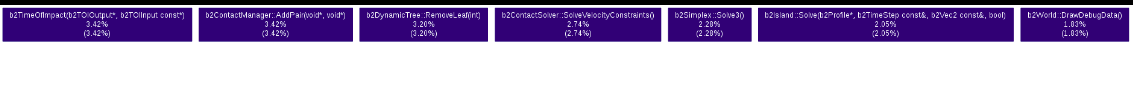
\includegraphics[scale=0.4]{release3.png}\newline
\small{release mode\\}
\end{center}


\begin{center}
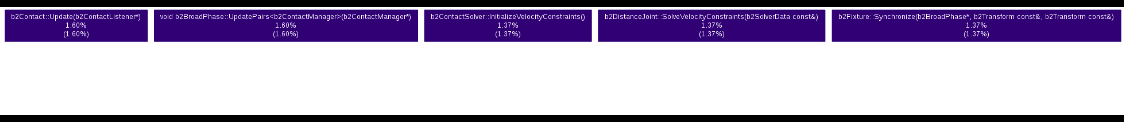
\includegraphics[scale=0.4]{release4.png}\newline
\small{release mode\\}
\end{center}


\begin{center}
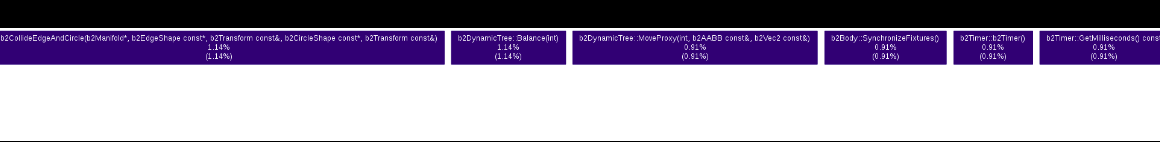
\includegraphics[scale=0.4]{release5.png}\newline
\small{release mode\\}
\end{center}


\begin{center}
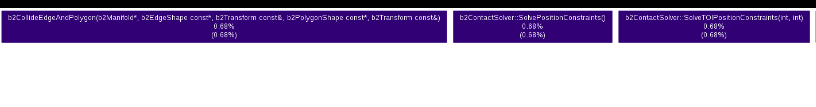
\includegraphics[scale=0.4]{release6.png}\newline
\small{release mode\\}
\end{center}

.
\begin{center}
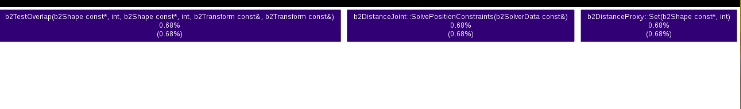
\includegraphics[scale=0.4]{release7.png}\newline
\small{release mode\\}
\end{center}

\newpage



\begin{center}

\huge{
\textbf{SRS\\}}
\end{center}
\Large
{
A Linux Operating Software such as Ubuntu.\\
A Box2D environment to run the applications.\\
}

\begin{center}

\huge{
\textbf{Work Distribution\\}}
\end{center}
\Large
{
Naveen Kumar(140050013):\newline
-Basic structure of the code\newline
-Creating callgraphs.\newline
-Handling makefile\newline
\newline

Yathansh Kathuria(140050021):\newline
-Responsible for the idea of simulating combustion engine\newline
-Beamer presentation\newline
-Web Page\newline
\newline

Rajat Chaturvedi\newline
-Debugging of code\newline
-Project report\newline
-Project video\newline
\newline
Note: All three group members were responsible for major ideas on how to go on with the project. Each member contributed to the success of the project. There were many times where a member's idea or insight helped us in going forward, and we won't be able to list them all.
\newline
}




\begin{center}

\huge{
\textbf{Link To Webpage\\}}
\end{center}
\Large
{
\url{www.cse.iitb.ac.in/~knaveen/box2d.html}
}




\begin{thebibliography}{9}
\bibitem{ref1}
Box2D 4-Stroke Combustion Engine
\url{https://www.youtube.com/watch?v=8kZRpouZ3OQ}

\bibitem{ref2}
Box2D mannual
\url{http://www.box2d.org/manual.html}

\bibitem{ref3}
Box2D Tutorial
\url{http://www.iforce2d.net/b2dtut/}

\bibitem{ref4}
Box2D Blog
\url{http://codingowl.com/readblog.php?blogid=119}

\bibitem{ref5}
Making Repository
\url{http://github.com/}

\bibitem{ref6}
doxygen tutorial
\url{https://www.stack.nl/~dimitri/doxygen/manual/}

\bibitem{ref7}
Non Convex Shape Box2D
\url{http://www.emanueleferonato.com/2011/09/12/create-non-convex-complex-shapes-with-box2d/}

\bibitem{ref8}
Bibliography
\url{https://www.sharelatex.com/learn/Bibliography_management_with_bibtex}

\bibitem{ref9}
git tutorial
\url{https://www.atlassian.com/git/tutorials/undoing-changes/git-checkout}

\bibitem{ref10}
youtube video
\url{https://www.youtube.com/watch?v=QPaUJfA1KsY}

\bibitem{ref11}
\url{piazza.com}

\bibitem{ref12}
tutorial for webpage
\url{w3school.com}

\bibitem{ref13}
video making software- kazam
\url{https://apps.ubuntu.com/cat/applications/kazam/}












\end{thebibliography}


\end{document}
